\chapter{State of the art}

In questo capitolo saranno inizialmente esposti i concetti teorici alla base dell'applicazione 
sviluppata: dagli algoritmi più comuni per la \textbf{Face Detection} 
ad un'introduzione al \textbf{Machine Learning} per finire
poi con elementi di \textbf{Programmazione Lineare Multiobiettivo}.

Verranno quindi analizzati precedenti progetti che hanno affrontato le stesse problematiche.

\section{Face Detection}

La Face Detection è una tecnologia
che permette di localizzare ed estrarre da un'immagine la regione contenente un 
volto \cite{Datta2015}; ha oggigiorno diverse applicazioni ed utilizzi, dal 
video coding al content-based image retrieval. 

\begin{figure}
    \begin{small}
        \begin{center}
            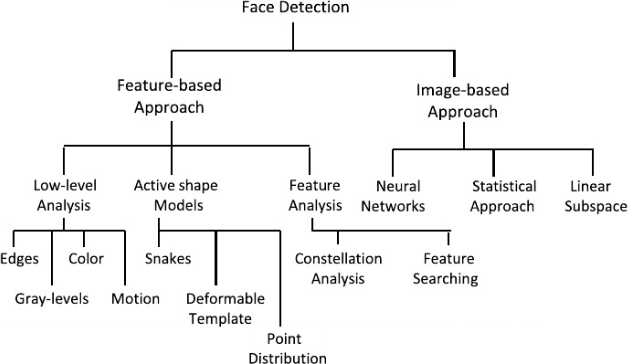
\includegraphics[width=0.95\textwidth]{face_detection_techniques.png}
        \end{center}
        \caption{Diversi approcci alla face detection}
        \label{fig:face_detection_approaches}
    \end{small}
\end{figure}

\subsection{Problematiche comuni}

Le sfide che una tecnica di face detection si trova ad affrontare sono solitamente 
(\cite{Datta2015}):

\begin{itemize}
    \item \textbf{Occlusione}. Spesso parte dei volti sono nascosti da oggetti e/o 
        altri volti
    \item \textbf{Espressioni}. L'aspetto dei volti è fortemente influenzato 
        dall'espressione della persona.
    \item \textbf{Posa}. La posizione da cui è scattata l'immagine influenza la 
        prospettiva del volto (\ref{fig:fd_problem}).
    \item \textbf{Luminosità}. Livelli di luminosità eccessivi o troppo bassi 
        impediscono di ricoscere contorni e linee del viso.
\end{itemize}

\begin{figure}
    \begin{small}
        \begin{center}
            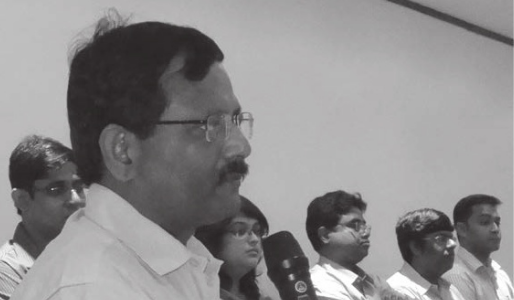
\includegraphics[width=0.50\textwidth]{face_detection_situation.png}
        \end{center}
        \caption{Un classico esempio di problema di face detection}
        \label{fig:fd_problem}
    \end{small}
\end{figure}

\subsection{Approcci feature-based}

In un periodo di ricerca che coinvolge circa gli ultimi trenta anni sono state 
usati diversi approcci che permettessero di sviluppare tecniche di face detection
(\ref{fig:face_detection_approaches}), dividendosi principalmente in due categorie: 
\textbf{Feature-based} e \textbf{Image-based}.

Nei primi vengono solitamente estratte le feature di un volto da 
un'immagine (come ad esempio occhi, labbra, sopracciglia) per poi verificare, 
attraverso la relazione che persiste tra di loro, la presenza di un volto.

All'interno di questa categoria possono essere indivuate ulteriori distinzioni
(\cite{Datta2015}, 2.2):

\begin{itemize}
    \item \textbf{Low Level Analysis}. Feature vengono estratte basandosi sulle 
        proprietà dei pixel come ad esempio colore o valore nella scala di grigi.
    \item \textbf{Feature Analysis}. Vengono sfruttate le proprietà geometrice 
        del volto per cercare di localizzare ed individuare le diverse parti del viso.
    \item \textbf{Active shape models}. Questi modelli, che vanno da \textit{snakes}
        ai PDM (point-distributed models) sono usati per l'estrazione di feature 
        complesse e per tracciare le iridi degli occhi e le labbra.  
\end{itemize}

\subsection{Algoritmo Viola-Jones per la Face Detection}

Invece tra gli svariati approcci \textbf{Image-based} uno che ha avuto particolare successo, soprattutto per la 
velocità di calcolo che permette il suo utilizzo in applicazioni che utilizzano grandi 
moli e flussi di immagini, è l'algoritmo Viola-Jones.

\medskip

Esso fa uso di Haar functions per il l'individuazione delle features, i.e. 
si basa sul calcolo della somma e differenza di pixel in particolari rettangoli 
\cite{Viola2004}, come mostrato in \ref{fig:haar}.

Il calcolo viene enormemente velocizzato attraverso le \textit{integral images}, 
immagini in cui il valore dei pixel è pari alla somma dei pixel in alto a sinistra, i.e.

\begin{equation}
    ii(x,y) = \sum_{x'\leq x, y' \leq y}^{} i(x', y')
    \label{eq:}
\end{equation}

con $ii(x,y)$ il valore del pixel nella \textit{integral image} e $i(x',y')$ 
il valore nell'immagine originale.

\begin{figure}
    \begin{small}
        \begin{center}
            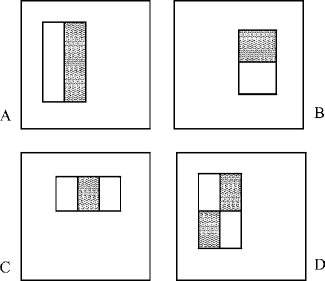
\includegraphics[width=0.40\textwidth]{haar_example.png}
        \end{center}
        \caption{Al valore dei pixel nella regione bianca viene sottratto il valore nella regione scura}
        \label{fig:haar}
    \end{small}
\end{figure}

\medskip

Tali \textit{Haar functions} vengono usate quindi da \textbf{classificatori}, 
delle funzioni che mappano un'osservazione (in questo caso un insieme di pixel) su un un set finito di valori, 
in questo caso \cite{Wang2014}
$f:$\Rset$^d\rightarrow \{-1, 1\}$.

Attraverso un Ada Boosting questi singoli ed imprecisi classificatori vengono combinati tra di loro
per ottenere un classificatore "forte" che risulta essere molto più accurato \cite{Schapire2013} dei singoli.

Dato un esempio da classificare $x$, l'esito della classificazione "forte" è pari a 

\begin{equation}
    F(x) = \sum_{t=1}^{T} \alpha_t h_t(x)
    \label{eq:}
\end{equation}

con $h_t(x)$ classificatore "debole" a cui corrisponde un peso "di voto" pari a $\alpha_t$:
il risultato è quindi ottenuto come la maggioranza pesata delle classificazioni deboli.

\medskip

Il rendimento può essere ulteriormente migliorato con l'utilizzo di classificatori a cascata 
(\ref{fig:cascade}). Un classificatore a cascata è costituito da diversi \textit{stages}, 
ognuno contenente uno classificatore "forte", ciascuno dei quali determina se la finestra in 
input non contiente sicuramente un volto oppure potrebbe. Quando viene predetta l'assenza 
certa di un viso l'immagine viene scartata, altrimenti è passata allo \textit{stage} successivo 
\cite{Datta2015}.

\begin{figure}
    \begin{small}
        \begin{center}
            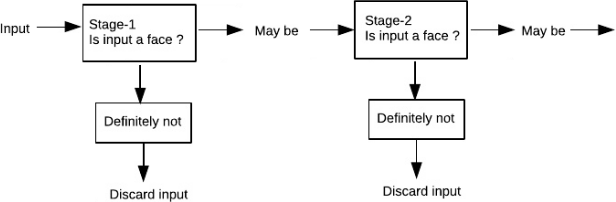
\includegraphics[width=0.95\textwidth]{cascade.png}
        \end{center}
        \caption{Struttura dei classificatori a cascata}
        \label{fig:cascade}
    \end{small}
\end{figure}

\newpage

\section{Regressioni e Machine Learning}

La regressione è una tecnica statistica utilizzata per determinare la relazione che persiste tra
due o più variabili: essa è principalmente adoperata per predizioni e inferenze.

Nella sua forma più semplice (bivariata) la regressione mostra la relazione tra una variabile 
indipendente $X$ ed una variabile dipendente, $Y$, attraverso un'equazione del tipo

\begin{equation}
    Y = \beta_0 + \beta_1 X + u
    \label{eq:biv_regression}
\end{equation}

La regressione riesce quindi a quantificare quanto la variazione di una variabile è dipendente 
dalla variazione di un'altra; quello che invece la non è capace di dimostrare è la casualità, 
la quale è dimostrata solo analiticamente \cite{campbell2008introduction}.

\begin{figure}[bh]
    \begin{small}
        \begin{center}
            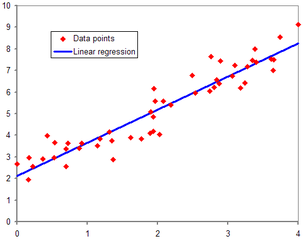
\includegraphics[width=0.50\textwidth]{regression.png}
        \end{center}
        \caption{Un esempio di utilizzo di regressione lineare: la retta cerca 
            di stimare la relazione tra le due grandezze raffigurate}
        \label{fig:}
    \end{small}
\end{figure}

\subsection{Reti neurali}

Negli ultimi decenni il Machine Learning è diventato uno dei principali strumenti utilizzati in 
ambito informatico grazie alla grande mole di dati che è possibile ormai raccogliere e si può 
addirittura pensare che il suo influsso negli prossimi anni si accrescerà ulteriormente \cite{Smola2008}.

In questo ambito ricoprono grande importanza le reti neurali, un tecnologia che che si è rivelata
molto adatta all'individuazione ed al riconoscimento di pattern statistici \cite{bishop2006pattern},
in particolare i \textit{multilayer perceptron}, i quali si basano sulla combinazione di una serie di funzioni con pesi variabili.

\begin{figure}
    \begin{small}
        \begin{center}
            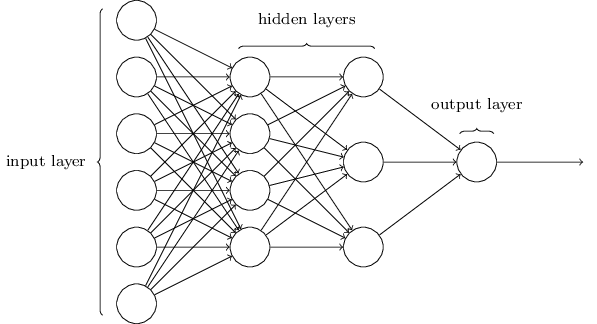
\includegraphics[width=0.95\textwidth]{perceptron_network.png}
        \end{center}
        \caption{Un esempio di rete neurale \textit{multilayer perceptron} in cui è 
            possibile distinguere diversi livelli di nodi: un livello di input, 
            due layer nascosti ed uno di output}
        \label{fig:nn}
    \end{small}
\end{figure}

In ciascuno dei nodi del primo livello ad esempio (come mostrato in \ref{fig:nn}) viene calcolato un certo valore 
di attivazione pari a 

\begin{equation}
    a_j = \sum_{i=1}^{D} w_{ij}^{(1)} x_i + w_{j0}^{(1)}
    \label{eq:node_nn}
\end{equation}

con D numero di ingressi della rete, $x_i$ valore dell'input i-esimo; i $w_{j0}^{(1)}$, chiamati \textit{bias}, sono coefficienti fissati
del primo layer e 
$w_{ij}^{(1)}$, chiamati \textit{weights}, coefficienti che verranno modificati per adattarsi al modello che dovranno stimare.

L'output del nodo j-esimo (che verrà in seguito utilizzato come precedentemente era stato fatto con gli input) sarà quindi
\cite{bishop2006pattern}

\begin{equation}
    z_j = h(a_j)
    \label{eq:activation}
\end{equation}

con $h()$ funzione non lineare definita \textit{activation function}, che solitamente corrisponde ad una $tanh$, ad una 
ReLU, definita come \cite{Nwankpa2018}

\begin{equation}
    ReLU(x) = \max (x, 0)
    \label{eq:relu}
\end{equation}

\noindent
oppure ad una sigmoide \cite{Nwankpa2018}

\begin{equation}
    \sigma(x) = \frac{1}{1+e^{-x}}
    \label{eq:sigmoid}
\end{equation}


Nel layer finale questa funzione di attivazione varia a seconda della tipologia di problema: nel caso di regressione 
corrisponde all'identità, 
viceversa nella classificazione viene spesso usata una softmax \cite{Keck2014}, che restituisce per 
l'elemento in posizione $j$ nel layer di output 

\begin{equation}
    \mathbf{\sigma(z)}_j = \frac{e^{z_j}}{\sum_{k=1}^{K}e^{z_k}}
    \label{eq:softmax}
\end{equation}

\begin{figure}[h]
    \begin{small}
        \begin{center}
            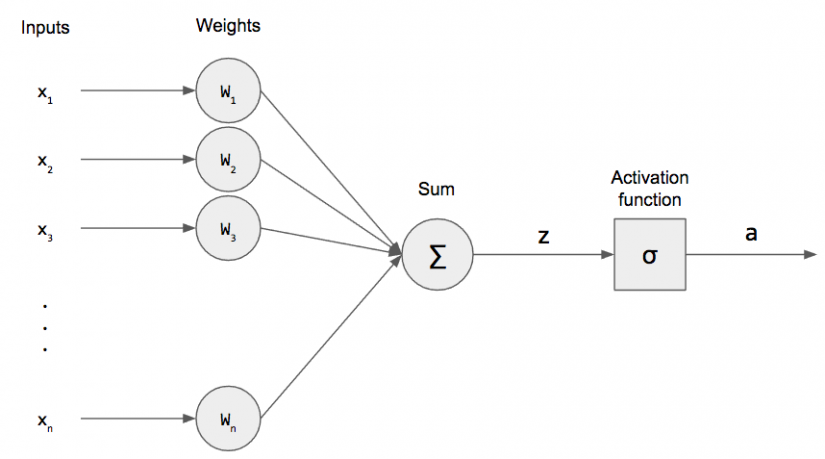
\includegraphics[width=0.70\textwidth]{single_perceptron.png}
        \end{center}
        \caption{Le operazioni algebriche per il calcolo dell'output di un singolo nodo}
        \label{fig:}
    \end{small}
\end{figure}

\subsubsection{Backpropagation} 

Fase fondamentale per una rete neurale è quella nella quale vengono analizzati i dati a disposizione 
(\textit{training}): è questa la fase nella quale, attraverso la cosiddetta \textit{backpropagation}, 
i pesi vengono adattati al problema in questione.

Questo corrisponde a cercare di minimizzare la seguente funzione di errore \cite{bishop2006pattern}

\begin{equation}
    E(\mathbf{w}) = \frac{1}{2} \sum_{n=1}^{N} || \mathbf{y(x_n, w) - t_n} || ^2
    \label{eq:error_nn}
\end{equation}

con $\mathbf{y(x_n, w)}$ output della rete e $\mathbf{t_n}$ target.

Questo miglioramento della rete viene effettuato modificando i pesi delle funzioni 
precedentemente definite, propagando all'indietro nella rete neurale il valore dell'errore:
viene calcolata la dipendenza dell'errore da ciascuno dei pesi, i.e.

\begin{equation}
    \frac{\partial E}{\partial w_{ij}} 
    \label{eq:err_nn}
\end{equation}

Che viene quindi utilizzato per modificare i pesi nel seguente modo \cite{Mazur2015}

\begin{equation}
    w_{ij}' = w_{ij} - \eta  \frac{\partial E}{\partial w_{ij}}
    \label{eq:back_err}
\end{equation}

\noindent
con $\eta$ \textit{learning step}, un parametro definito inizialmente.

\newpage

\section{Programmazione lineare}

La programmazione matematica studia la teoria ed i metodi utili per la ricerca 
di massimi o minimi di una funzione matematica, i.e. problemi del tipo 
\cite{walsh1985introduction}

\begin{center}
    minimizzare (o massimizzare) $f(x_1, \dots, x_n)$ soggetta a $(x_1, \dots, x_n)$ in $X$    
\end{center}

All'interno di essa ricopre 
grande importanza la programmazione lineare, che si occupa in particolare di risolvere 
problemi i cui vincoli e la funzione da minimizzare o massimizzare (detta 
\textit{funzione obiettivo}) sono tutte relazioni lineari\cite{walsh1985introduction}.
Si può facilmente vedere come un generico problema di questo tipo, (ad esempio di minimizzazione) 
possa essere scritto nella forma\cite{1990}

\begin{equation*}
    \min f(x)
    \label{eq:}
\end{equation*}
\begin{equation*}
    Ax \geq b, x \geq 0
    \label{eq:}
\end{equation*}

\subsection{Programmazione lineare multiobiettivo}

Un'ulteriore classe di problemi di programmazione matematica è costituita dai cosidetti
problemi multiobiettivo. In questo caso, denotando con 

\begin{equation*}
    \mathbf{\theta} = (\theta_1(x), \dots, \theta_p(x))
    \label{eq:}
\end{equation*}

il vettore delle p funzioni obiettivo, allora il problema consiste nel trovare le 
cosiddette soluzioni efficienti (o \textbf{ottimi di Pareto}), ovvero tutte $\bar{x}$ tali 
che non esiste $x$ ammissibile (cioè che rispetta tutti i vincoli) tale che 
$\mathbf{\theta}(x) \leq \mathbf{\theta}(\bar{x})$ (nel caso di minimo) e 
$x \neq \bar{x}$ \cite{walsh1985introduction}.

L'insieme di queste soluzioni viene solitamente definito \textbf{frontiera di Pareto}, 
ed essa è graficamente visibile se si rappresenta l'insieme dei valori ammissibili nello 
spazio degli obiettivi Y, cioè l'insieme dei valori assunti da tutte $x \in X$ 
(le $x$ ammissibili).

\begin{figure}
    \begin{small}
        \begin{center}
            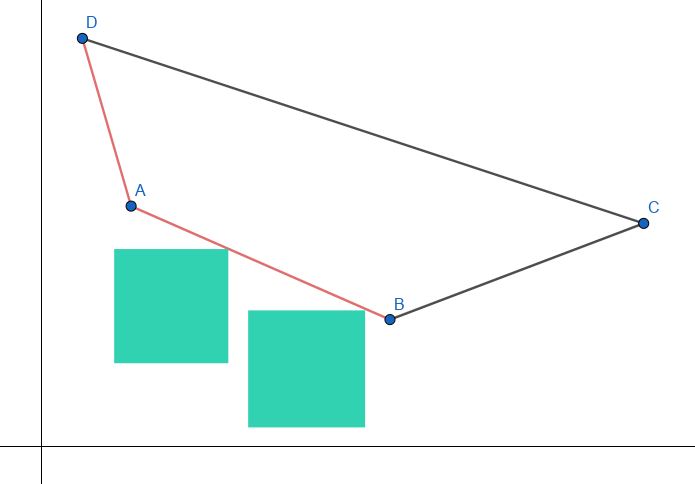
\includegraphics[width=0.70\textwidth]{multiobjective_example.png}
        \end{center}
        \caption{I segmenti in rosso rappresentano la frontiera di Pareto
            in un ipotetico problema di minimo: i punti da cui sono generati i 
            quadranti inferiori non contengono altri elementi dell'insieme 
            ammissibile nello spazio delle soluzioni}
        \label{fig:obj}
    \end{small}
\end{figure}

Nel caso di due funzioni obiettivo (Figure~\ref{fig:obj}) i punti appartenenti 
alla frontiera di Pareto sono facilmente verificabili attraverso la regola del quadrante
inferiore, cioè non vi devono essere elementi contenuti nel quadrante in basso a sinistra 
rispetto al punto considerato.

\subsubsection{Teorema di Geoffrion} 
Per il calcolo delle soluzioni efficienti si rivela molto utile il teorema di Geoffrion, il
quale enuncia che \cite{Figueira2006}, considerando il seguente problema multiobiettivo

\begin{equation*}
    \min (Cx)    
    \label{eq:}
\end{equation*}
\begin{equation}
    Ax \geq b, x \geq 0
    \label{eq:multi_problem}
\end{equation}

\noindent
con $C \in $\Rset$_{p \times n}$ matrice delle $p$ funzioni obiettivo,

allora una soluzione $x$ è un ottimo di Pareto $\iff \exists \lambda = (\lambda_1, \dots, 
\lambda_p) \geq 0$, $\sum_{i=1}^{p} \lambda_i = 1$ tale che $x$ è ottima per il seguente 
problema

\begin{equation*}
    \min (\lambda Cx)    
    \label{eq:}
\end{equation*}
\begin{equation*}
    Ax \geq b, x \geq 0
    \label{eq:}
\end{equation*}

\subsection{Programmazione lineare intera multiobiettivo}

Nel caso in cui il problema multiobiettivo ha l'ulteriore vincoli delle variabili intere,
allora per il calcolo della frontiera di Pareto (trasformando il problema in un singolo 
obiettivo, processo detto di \textit{scalarizzazione}) si può ricorrere a due diversi metodi: 
il \textbf{metodo dei pesi} oppure il metodo \textbf{$\epsilon$-constraints}. 

\subsubsection{Metodo dei pesi}

Il metodo dei pesi è il più noto metodo di scalarizzazione: esso consiste nel far variare 
$\lambda = (\lambda_1, \dots, \lambda_p) \geq 0$, con $\sum_{i=1}^{p} \lambda_i = 1$ trasformando 
\ref{eq:multi_problem} (dotato dell'ulteriore vincolo $x \in$ \Zset$^n$) in 

\begin{equation*}
    \min (\lambda Cx)    
    \label{eq:}
\end{equation*}
\begin{equation*}
    Ax \geq b, x\geq 0
    \label{eq:}
\end{equation*}

E' importante però notare che questo metodo non permette di calcolare tutta la frontiera di Pareto:
esso genere solo un sottoinsieme di punti che si definisce \textbf{supportato}. 

\subsubsection{Metodo $\epsilon$-constraints}

In questo caso una sola delle $p$ funzioni obiettivo rimane tale mentre le altre sono trasformate in 
dei vincoli \cite{Figueira2006}.

Il problema è quindi riformulato nella forma (per $x \in$ \Zset$^n$)

\begin{equation*}
    \min (c_kx)    
    \label{eq:}
\end{equation*}
\begin{equation*}
    \min (c_ix \leq \epsilon_i)  \quad \forall i \in \{1, \dots, p\}, i \neq k   
    \label{eq:}
\end{equation*}
\begin{equation*}
    Ax \geq 0, x \geq 0
    \label{eq:}
\end{equation*}

A differenza del metodo dei pesi, riesce a generare tutte le soluzioni efficienti.
